\title{Architectural Views}
\maketitle

\section{Introduction}

Understanding software is hard.
It is often claimed that reading code is harder than writing code.
This principle is used to explain a programmers innate desire to constantly rewrite their code from scratch.
If software is hard to understand than software architecture is near impossible.
Fortunately, architects have developed a number of techniques to manage this complexity.

A software architecture consists of many dimensions.
Programming languages, communication protocols, the operating systems and hardware used, virtualisation used,
and the code itself are a subset of the many dimensions which comprise a software architecture.
Asking a programmers monkey brain to understand, communicate, or document every dimension at once is needlessly cruel.
This is where architectural views come in.

Architectural views, or architectural projections, are a representation of one or more related aspects of a software architecture.
Views allow us to focus on a particular slice of our multi-dimensional software architecture, ignoring other irrelevant slices.
For example, if we're interesting in applying a security patch in our software then we're only interested in the view
which tells us which software packages are used on each host machine.

The successful implementation of any architecture relies on the ability for the architectural views
to be disseminated, understood, and implemented.
For some institutions, the software is simple enough, or the team small enough, that the design
can be communicated through word of mouth.
As software becomes increasingly complex and developers number in the thousands,
it is critical for design to be communicated as effectively as possible.
In addition to facilitating communication,
architectural views also enable architectural policies to be designed and implemented.

The seminal architecture book, Software Architecture in Practice \cite{bass2013software},
categorises architectural views into three groups.
These three groups each answer different questions about the architecture, specifically:
\begin{description}
    \item[Module Views] How implementation components of a system are structured and depended upon.
    \item[Component-and-connector Views] How individual components communicate with each other.
    \item[Allocation Views] How the components are deployed to hardware.
\end{description}

\section{Module Views}
Module views are composed of modules, which are static units of functionality such as classes, functions, modules, or whole programs.
The defining characteristic of a module is that it represents software responsible for some well-defined functionality.
For example, a class which converts JSON to XML would be considered a module, as would a function which performs the same task.

The primary function of module views are to communicate the dependencies of a module.
Rarely does software work completely in isolation, often is it constructed with implicit or explicit dependencies.
A module which converts JSON to XML might depend upon a module which parses JSON and a module which can format XML.
Module views make these dependencies explicit.

\begin{figure}[ht]
\centering
\begin{subfigure}[b]{\textwidth}
\begin{shaded}
\begin{lstlisting}[style=python]
import json
import xml

class JSONtoXML:
    def load(self, json_file):
        with open(json_file) as f:
            data = json.load(f)
        self.data = self.convert(data)

    def export(self, xml_file):
        xml.write(xml_file, data)

    def convert(self, data: JSON) -> XML:
        ...
\end{lstlisting}
\end{shaded}
\caption{Pseudo-code to convert JSON to XML}
\end{subfigure}


\begin{subfigure}[b]{\textwidth}
\begin{center}
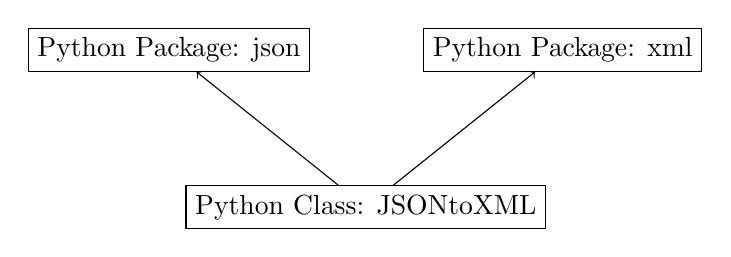
\begin{tikzpicture}
    \node[draw] (json) at (0,0) {Python Package: json};
    \node[draw] (xml) at (5,0) {Python Package: xml};
    \node[draw] (jsontoxml) at (2.5,-2) {Python Class: JSONtoXML};

    \path [->] (jsontoxml) edge node {} (json);
    \path [->] (jsontoxml) edge node {} (xml);
\end{tikzpicture}
\end{center}
\caption{An example of a module view which illustrates the dependencies of the \texttt{JSONtoXML} class}
\end{subfigure}
\caption{A simple module view of a JSON to XML program.}
\end{figure}

\section{Component-and-connector Views}
Component-and-connector views focus on the runtime, or dynamic behaviour of a system.
Components are units which perform some computation or operation at runtime.
These components could overlap with the modules of a module view but are often at a higher level of abstraction.
The focus of component-and-connector views is how these components communicate at runtime.
Runtime communication is the connector of components.
For example, a service which registers users to a website might have new registrations communicated via a REST request.
The service may then communicate the new user information to a database via SQL queries.

When we look at software architecture, component-and-connector views are the most commonly used views.
They are common because they contain runtime information which is not easily automatically extracted.
Module views can be generated after the fact, i.e. it is easy enough for a project to generate a UML inheritance diagram.
Component-and-connector views are often something that is maintained manually by architects and developers.
